\lecture{Introduzione a Industrial Robotics}{31~-~05~-~2026}
%
\section{Definizio e concetti fondamentali}
La Robotica Industriale è la disciplina ingegneristica che si occupa di progettazione, controllo e applicazione di dispositivi meccanici programmabili. Si concentra su compiti ripetitivi, pericolosi o di precisione (es. saldatura, assemblaggio).
%
\paragraph{Definizione ISO di Robot} Un robot è un manipolatore multiscopo, riprogrammabile (il compito può essere cambiato senza modifiche fisiche) e controllato automaticamente, dotato di tre o più assi.
%
\paragraph{Automazione tradizione vs Robot} A differenza dell'automazione rigida (dedicata meccanicamente a un singolo compito), i robot offrono flessibilità, tempi di cambio formato più brevi e integrazione con sensori.

\begin{recall}[Gradi di libertà]
    Un corpo rigido nello spazio 3D ha esattamente 6 gradi di libertà: 3 traslazioni (lungo gli assi x, y, z) e 3 rotazioni (attorno agli assi x, y, z). I manipolatori industriali comuni hanno 6 \emphtb{DoF} (Degrees of Freedom) proprio per poter controllare in modo completo sia la posizione che l'orientamento dello strumento. Vedi figura \ref{fig:dof}.
    \begin{figure}
        \centering
        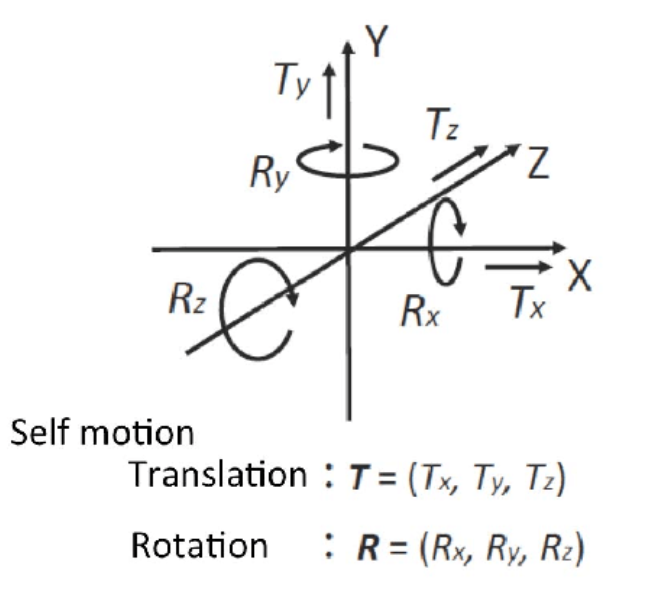
\includegraphics[width=0.5\linewidth]{assets/dof.png}
        \caption{Degrees of Freedom}\label{fig:dof}
    \end{figure}
\end{recall}

%
\subsection{Pose of a rigid body}
La posa (\emph{pose}) È la combinazione di Posizione (le coordinate x, y, z di un punto) e Orientamento (la rotazione rispetto a un sistema di riferimento). La posa del robot richiede quindi 6 parametri per essere descritta in uno spazio 3D. Vedi figura \ref{fig:pose}.
\begin{figure}
    \centering
    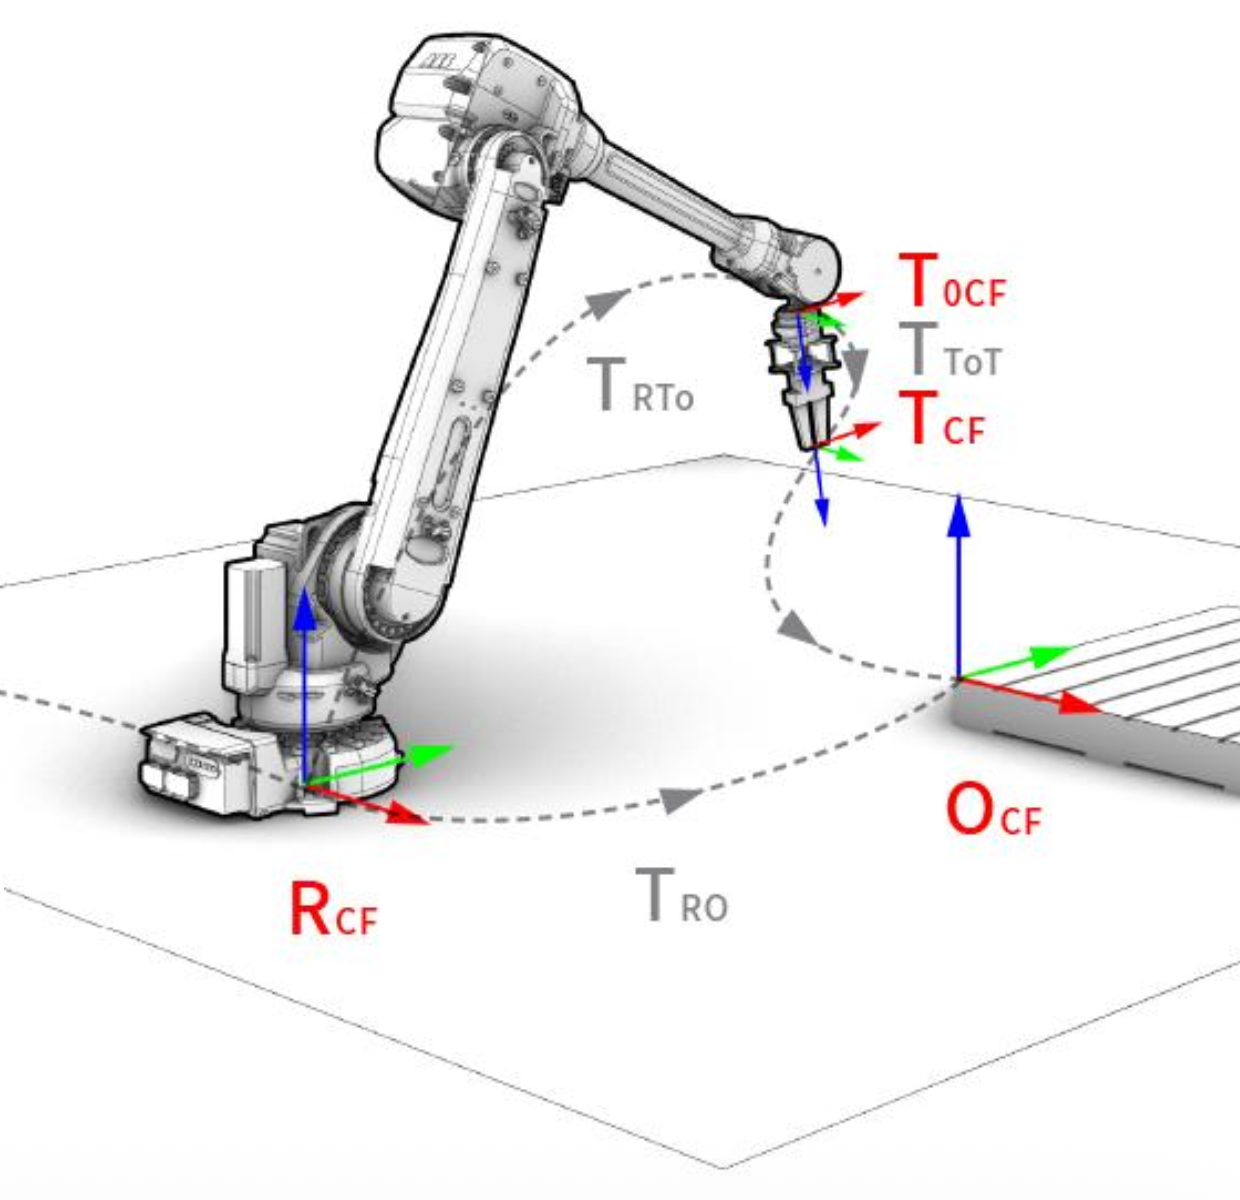
\includegraphics[width=0.5\linewidth]{assets/pose.png}
    \caption{Pose of a rigid body}\label{fig:pose}
\end{figure}

%
\section{Componenti meccanici e Parametri di prestazione}
\paragraph{Terminologia strutturale}
\begin{itemize}
    \item \textbf{Link}: Membro rigido che collega due giunti.
    \item \textbf{End-effector / Tool}: Il dispositivo posto all'estremità del braccio (es. pinza, pistola a spruzzo).
    \item \textbf{TCP (Tool Center Point)}: Il punto di riferimento associato allo strumento finale, essenziale per definire il posizionamento.
\end{itemize}
%
\paragraph{Joints}
Vi sono varie tipologie di giunti:
\begin{enumerate}
    \item \emphtb{Giunto Rotoide} (R): Produce una rotazione attorno a un asse (molto comune nei robot articolati e SCARA).
    \item \emphtb{Giunto Prismatico} (P): Produce una traslazione lineare lungo un asse (usato nei robot cartesiani).
\end{enumerate}
%
\paragraph{Metriche di prestazione}
\begin{itemize}
    \item \textbf{Ripetibilità vs Accuratezza}
          \begin{itemize}
              \item \emph{Accuratezza}: È la differenza tra la posa comandata e la vera posa raggiunta dal robot.
              \item \emph{Ripetibilità}: È la capacità del robot di ritornare esattamente alla stessa posa comandata più volte. I robot industriali tipicamente mostrano un'alta ripetibilità ma un'accuratezza assoluta più moderata.
          \end{itemize}
    \item \textbf{Spazio di lavoro (Workspace)}: La regione di spazio che il TCP può raggiungere.
    \item \textbf{Payload}: Carico massimo che il braccio può trasportare ad una certa velocità.
\end{itemize}

\begin{figure}
    \centering
    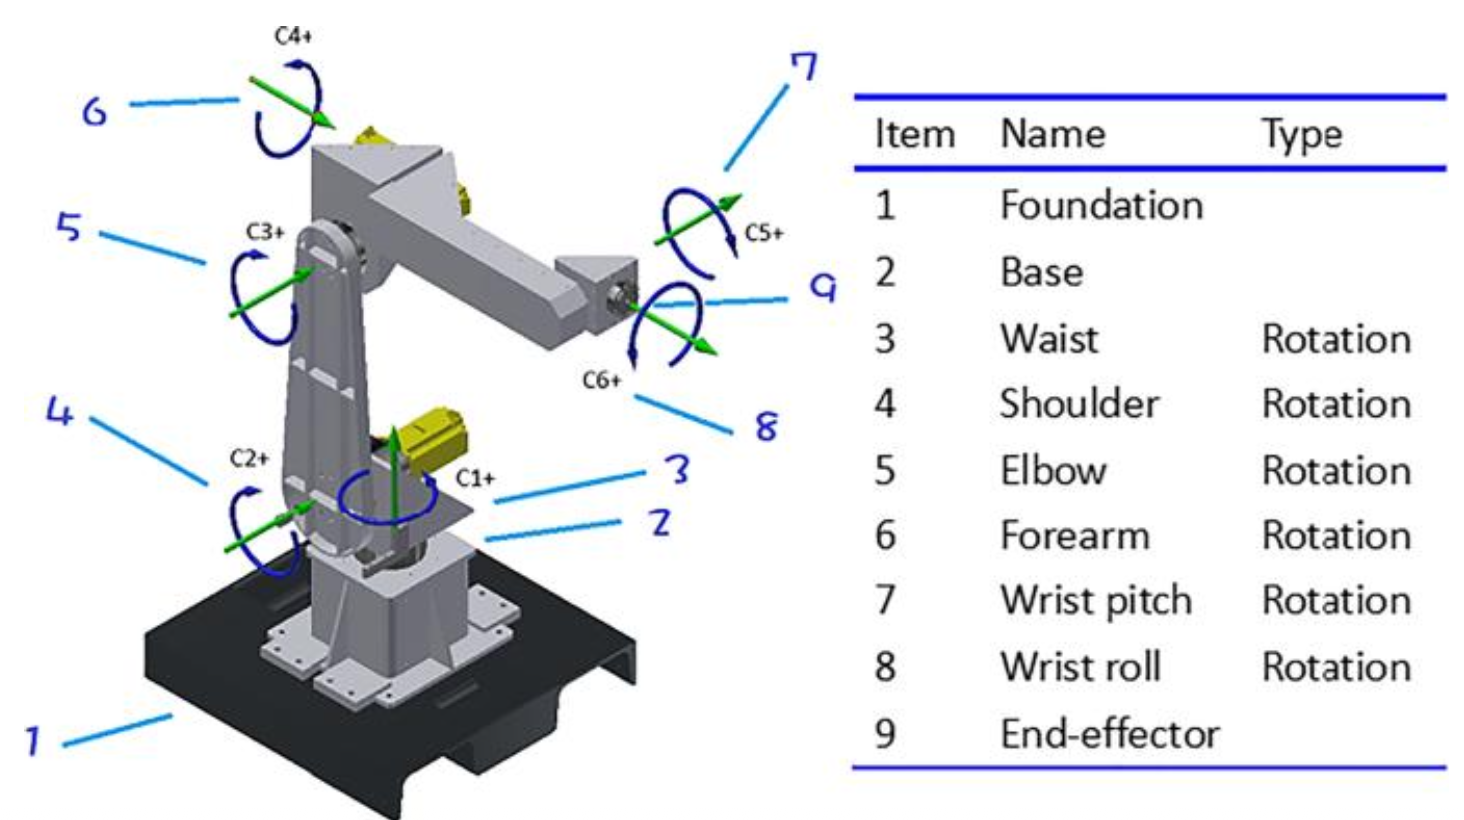
\includegraphics[width=\linewidth]{assets/robot.png}
    \caption{Definition of a robot (standards)}\label{fig:rob}
\end{figure}

%
\section{Tipologie di Robot Industriali}
%
\subsection{Robot Cartesiani / Gantry}
Strutturati con tre giunti prismatici lungo assi ortogonali (X, Y, Z). Offrono alta rigidità, grande spazio di lavoro rettangolare ed elevata accuratezza. Sono usati per carichi pesanti e macchine CNC.
%
\subsection{Robot SCARA}
Hanno 2 o 3 giunti rotanti sul piano orizzontale e un asse prismatico verticale. Sono rigidi verticalmente ma cedevoli orizzontalmente. Sono estremamente veloci per movimenti brevi planari, ideali per assemblaggio e pick-and-place leggero.
%
\subsection{Robot Articolati (6 assi)}
Hanno una serie di giunti rotanti che ricordano un braccio umano. Il vantaggio principale è il controllo completo a 6 DoF e un ampio spazio di lavoro flessibile (possono aggirare gli ostacoli). Sono usati per compiti 3D complessi come saldatura e verniciatura, sebbene siano più lenti degli SCARA nei cicli brevi.
%
\subsection{Robot Delta / Paralleli}
Composti da bracci leggeri connessi in parallelo tra una base fissa e una piattaforma mobile. Avendo una massa in movimento bassissima, raggiungono velocità e accelerazioni estreme. Sono la scelta ideale per il pick-and-place ad alta velocità di oggetti leggeri (es. settore alimentare o farmaceutico).
%
\subsection{Robot Collaborativi (Cobot)}
Progettati per collaborare in sicurezza con gli umani nello stesso spazio. Hanno forme arrotondate, forza limitata e sensori di rilevamento. Il compromesso è che sono più lenti e hanno una capacità di carico (payload) inferiore rispetto ai robot tradizionali.

%
\section{Concetti di programmazione dei Robot}
%
\paragraph{Spazi di Movimento} Esiste lo spazio dei giunti (Joint space) e lo spazio del compito (Cartesian space).
%
\paragraph{Metodi di programmazione}
\begin{itemize}
    \item Online: Utilizza un ``teach pendant'' per registrare fisicamente i punti e i percorsi.
    \item Offline: Utilizza software di simulazione e CAD.
\end{itemize}
%
\paragraph{Tipi di Movimento} Punto a punto (PTP), Lineare (LIN) e Circolare (CIRC).

%
\section{Quiz}
\begin{qst}{}{dof}
    Why do many industrial robots have 6 DoF?
\end{qst}